\section{Faisal Najib Abdullah / 1174042}

\subsection{Teori}
\begin{enumerate}
\item Jelaskan apa itu klasifikasi teks, sertakan gambar ilustrasi buatan sendiri.\par
klasifikasi teks adalah cara untuk memilah-milah teks berdasarkan parameter tertentu baik itu jenis teks atau jenis dari dokumen yang terdapat kumpulan teks didalamnya, sedangkan teks itu sndiri merupakan sekumpulan kata yang dapat dibaca. bisa berupa buku, majalah, rambu-rambu dan lain sebagainya.

\begin{figure}[ht]
\centering
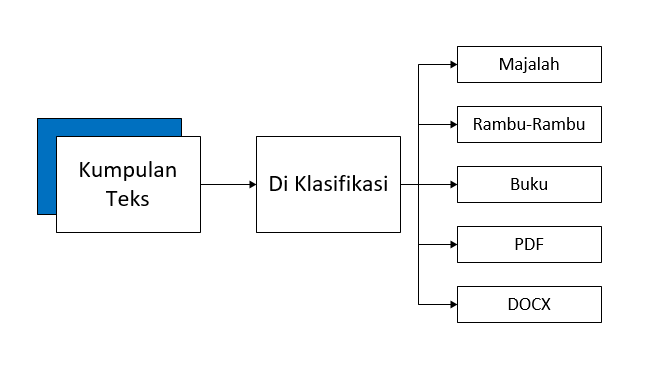
\includegraphics[scale=0.2]{figures/1174042/chapter4/1,1.PNG}
\caption{contoh klasifikasi teks}
\label{contoh}
\end{figure}

\item Jelaskan mengapa klasifikasi bunga tidak bisa menggunakan machine learning, sertakan ilustrasi sendiri.\par
Klasifikasi bunga tidakdapat menggunakan mesin learning dikarenakan jenis-jenis bunga banyak yang mirip bahkan banyak bunga yang serupa tetapi tidak sama. oleh karena itu klasifikasi bunga tidakbisa di gunakan oleh mesin learning dikarenakan jika salah satu inputan ciri-ciri dari siatu bunga di inputkan kemungkinan jawaban dari mesin learning itu tidak tepat contoh dimasukan inputan ciri ciri bunga mawar putih kemudian mesin learning menjawab bahwa itu bunga mawar merah.

\begin{figure}[ht]
\centering
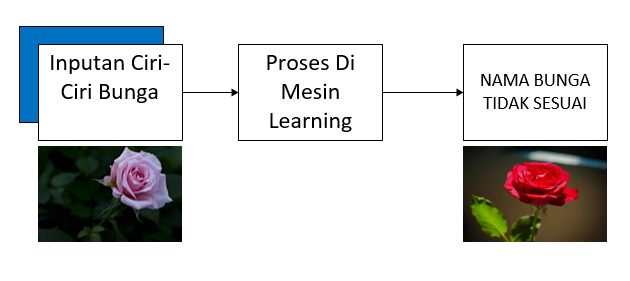
\includegraphics[scale=0.2]{figures/1174042/chapter4/1,2.PNG}
\caption{contoh klasifikasi bunga}
\label{contoh}
\end{figure}

\item Jelaskan bagaimana teknik pembelajaran mesin pada teks pada kata-kata yang digunakan di youtube,jelaskan arti per atribut data csv dan sertakan ilustrasi buatan sendiri.\par
cara pembelajaran teks yang di gunakan youtube yaitu dengan cara merekam data yang sering di inputkan oleh user pada menu pencarian youtube. sehingga pada saat user akan mencari data yang serupa seringkali youtube menyediakan opsi atau rekomendasi-rekomendasi dari pencaharian. contoh saya menuliskan m maka muncul opsi pilihan master chep dan lainya yang berawalan m rekomendasi yang muncul merupakan kata-kata yang sering di cari oleh banyak user atau sering di buka oleh user itu sendiri.

\begin{figure}[ht]
\centering
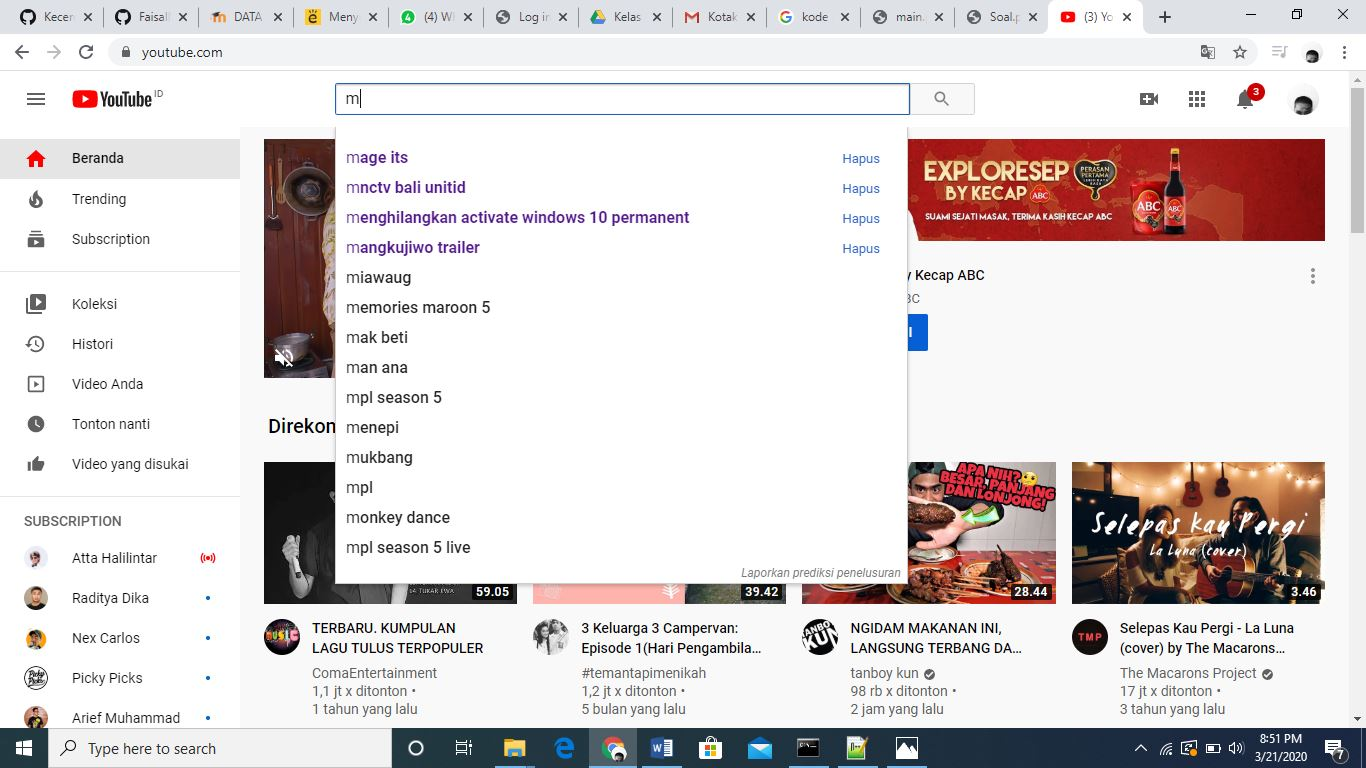
\includegraphics[scale=0.2]{figures/1174042/chapter4/1,3.JPG}
\caption{contoh teknik pembelajaran mesin}
\label{contoh}
\end{figure}

\item Jelaskan apa yang dimaksud vektorisasi data.\par
vektorisasi data merupakan pemechan data menjadi bagian bagian yang lebih sederhana contoh pada satu paragraf terdiri dari 200 kata kemudian dilakukan vektorisasi dengancara membagi-bagi kata dalam paragraf tersebut ke dalam kalimat-kalimat yang terpisah kemudian di pecah lagi menjadi data dalam perkata selanjutnya kata kata tersebut di terjemahkan.

\item Jelaskan apa itu bag of words dengan kata-kata yang sederhana dan ilustrasi sendiri.
 bag of words merupakan peroses penyederhanaan kata-kata yang asalnya tersiri dalam satu kalimat atau satu paragraf di ubah menjadi perkata kemudian kata-kata tersebut di kumpulkan menjadi satu kelompok tanpa ada arti dari kata-kata yang telah di kumpulkan tersebut lalu di hitung frekuensi kemunculan dari kata tersebut.
 
\begin{figure}[ht]
\centering
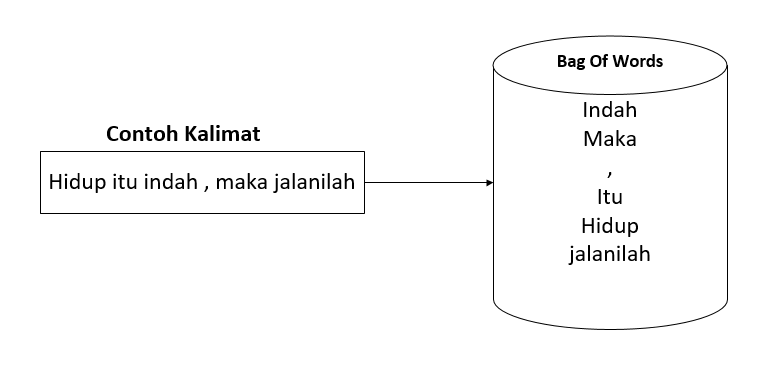
\includegraphics[scale=0.2]{figures/1174042/chapter4/1,5.PNG}
\caption{contoh bag of words}
\label{contoh}
\end{figure}

\item Jelaskan apa itu TF-IDF, ilustrasikan dengan gambar sendiri.
 TF-IDF merupakan metode untuk menghitung bobot dari kata yang sering muncul pada suatu kalimat. metode ini menghitung nilai TF atau Term Frequency dan IDF atau Inverse Document Frequency pada setiap kata pada kalimat yang dijadikan acuan kata pada metode ini sering di sebut token adapun rumus dari metode ini.
 
\begin{figure}[ht]
\centering
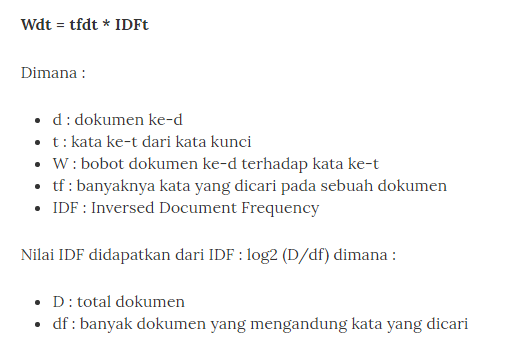
\includegraphics[scale=0.2]{figures/1174042/chapter4/1,6.PNG}
\caption{contoh TF-IDF}
\label{contoh}
\end{figure}

\end{enumerate}


\subsection{Praktek Program}
\begin{enumerate}
\item import data pandas dan 500 baris data dumy kemudian di jelaskan tiap barisnya.
\lstinputlisting{src/1174042/chapter4/2,1.py}
\begin{figure}[ht]
\centering
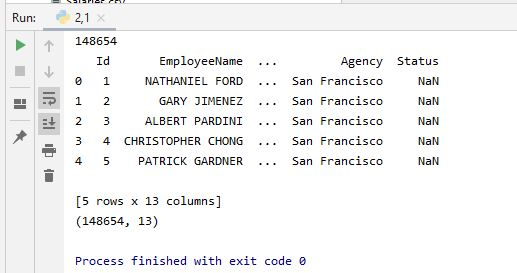
\includegraphics[scale=0.5]{figures/1174042/chapter4/2,1.JPG}
\caption{hasil}
\label{Praktek no 1}
\end{figure}

\item memecah data prame menjadi dua yag pertama 450 dan kedua sisanya
\lstinputlisting{src/1174042/chapter4/2,2.py}
\begin{figure}[ht]
\centering
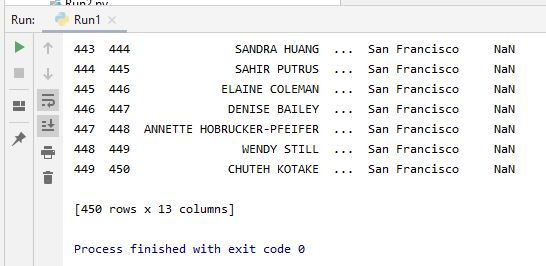
\includegraphics[scale=0.5]{figures/1174042/chapter4/2,2.JPG}
\caption{hasil}
\label{Praktek no 2}
\end{figure}

\begin{figure}[ht]
\centering
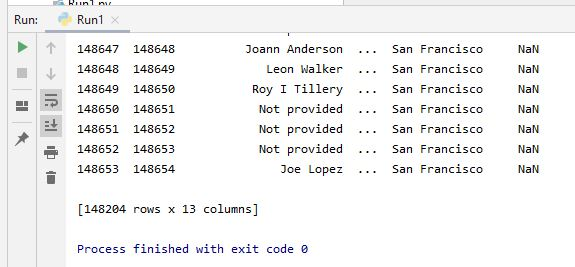
\includegraphics[scale=0.5]{figures/1174042/chapter4/2,2,1.JPG}
\caption{hasil}
\label{Praktek no 2}
\end{figure}

\item praktek vektorisasi\par
berikut merupakan codingan untuk melakukan vektorisasii data berupa teks dalam vormat csv
\lstinputlisting{src/1174042/chapter4/2,3.py}
\begin{figure}[ht]
\centering
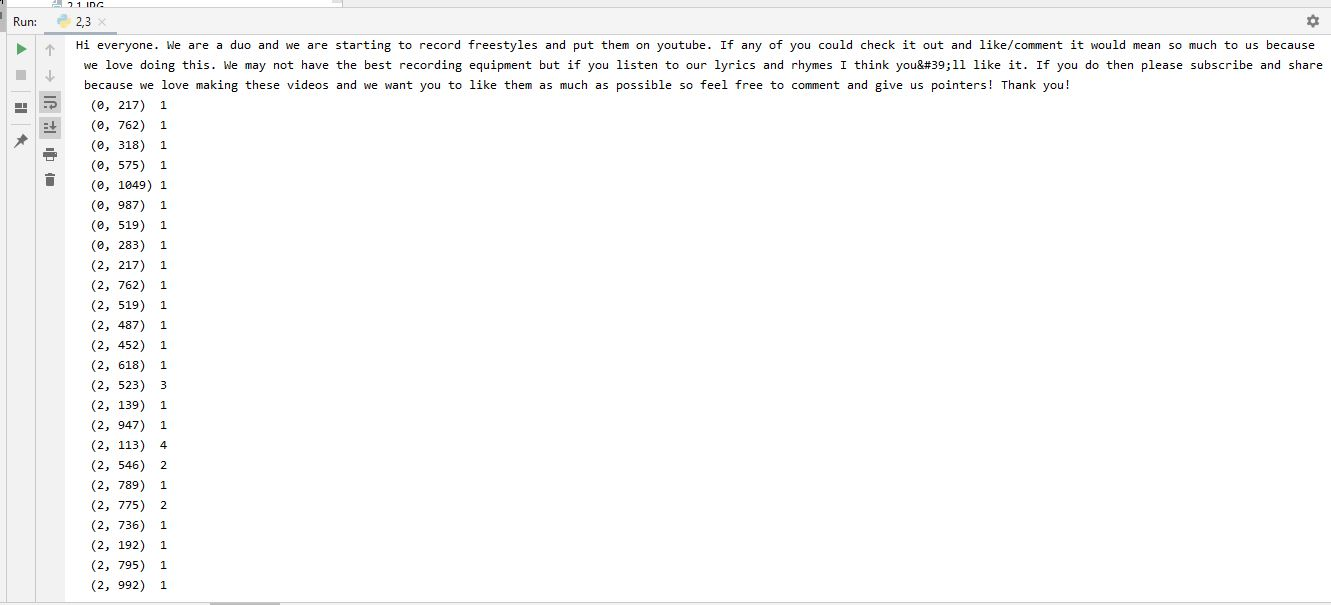
\includegraphics[scale=0.5]{figures/1174042/chapter4/2,3.JPG}
\caption{hasil}
\label{Praktek no 3}
\end{figure}
lakukan import library pandas yang di inisialisasi menjasi pd setelah itu ada dibuat class data\_komen dengan method read\_csv untuk membaca file berekstensikan csv yang di masukan alamatnya pada kurung, lakukan klasifikasi atau pemilihan komentar yang berisi spam atau bukan spam dengan parameter class samadengan 1 merupakan spam dan class samadengan 0 bukan spam setelah itu masukan librari CountVektorizer yang digunakan untuk vektorisasi data kemudian dilanjutkan pada bagian In[103] dibuat variabel yang berisi vektorisasi dari data pada data\_komen di field content setelah itu variabel tersebut di running hasilnya menunjukan 350 baris di kali 1738 kolom selanjutnya dicoba untuk memunculkan isi recod pada baris ke 349 maka akan muncul isian dari baris tersebut. selanjutnya dibuat variabel dk atau daftar yang berisi data hasil vektorisasi setelah yang terdiri dari variabel acak\_acak yang berisi data komen yang di dalamnya di buat random yang nantinya akan dibut data training dan data testing dengan ketentuan data training 300 dan data testing sebanyak 50 setelah itu data training di lakukan vektorisasi dan data testing juga dilakukan vektorisasi setelah itu kedua data training dan testing tersebut dibuat label dengan parameter field CLASS pada tabel.

\item klasifikasi SVM
berikut ini merupakan codingan klasifikasi SVM 
\lstinputlisting{src/1174042/chapter4/2,4.py}
\begin{figure}[ht]
\centering
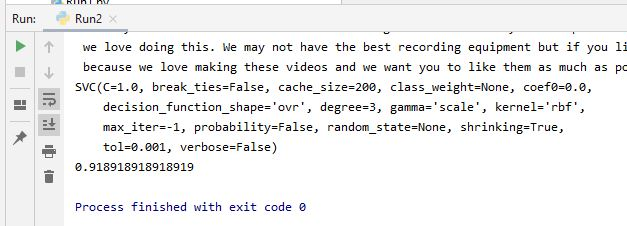
\includegraphics[scale=0.5]{figures/1174042/chapter4/2,4.JPG}
\caption{hasil}
\label{Praktek no 4}
\end{figure}
melakukan verifikasi import librari svm dari sklearn kemudian membuat variabel clfsvm berisikan method svc setelah itu variabel tersebut di berikan method fit dengan isian data train vektorisasi dan data training label yang berguna untuk melatih data tersebut setelah itu di coba untuk memunculkan score atau akurasi dari data tersebut menggunakan data testing vektorisasi dan data testing label.

\item klasifikasi decision tree 
berikut ini merupakan codingan klasifikasi decision tree
\lstinputlisting{src/1174042/chapter4/2,5.py}
\begin{figure}[ht]
\centering
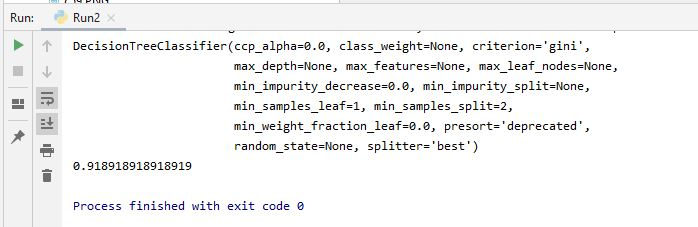
\includegraphics[scale=0.5]{figures/1174042/chapter4/2,5.JPG}
\caption{hasil}
\label{Praktek no 5}
\end{figure}
melakukan verifikasi import librari tree dari sklearn kemudian membuat variabel clftree berisikan method DecisionTreeClasifier setelah itu variabel tersebut di berikan method fit dengan isian data train vektorisasi dan data training label yang berguna untuk melatih data tersebut agar dapat digunakan pada codingan selanjutnya setelah itu di coba untuk memunculkan score atau akurasi dari data tersebut menggunakan data testing vektorisasi dan data testing label.

\item plot comfusion matrix
berikut merupakan codingan untuk confusion matrix 
\lstinputlisting{src/1174042/chapter4/2,6.py}
\begin{figure}[ht]
\centering
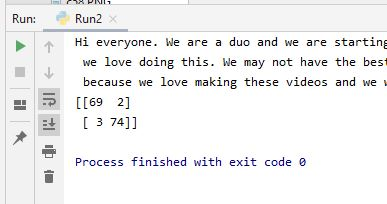
\includegraphics[scale=0.5]{figures/1174042/chapter4/2,6.JPG}
\caption{hasil}
\label{Praktek no 6}
\end{figure}
lakukan import library comfusion matrix selanjutnya dilakukan prediksi pada pada data tes nya kemudian data tersebut di masukan kedalam variabel cm dengan method confusion matrix yang di dalamnya terdapat data dari variabel perd label dan dk test label setelah itu variabel cm tersebut di running maka akan memunculkan nilai matrixnya. 

\item cross valodation 
berikut merupakan code untuk cross validation pada codingan pertama yaitu melakukan split 5 kali yaoti mengitung tingkat akurasi menggunakan data training.
\lstinputlisting{src/1174042/chapter4/2,7.py}
\begin{figure}[ht]
\centering
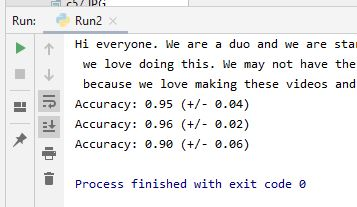
\includegraphics[scale=0.5]{figures/1174042/chapter4/2,7.JPG}
\caption{hasil}
\label{Praktek no 7}
\end{figure}
memunculkan nilai akurasi dari tiga metode yaitu random forest, decision tree, dan klasifikasi svm (suport vector machine) diamana akan di bandingkan tingkat akurasi dari semua hasil akurasiya mana yang terbaik dan lebih akurat pada hasilnya data yang paling akurat yaitu random forest.

\item Pengamatan program 
\lstinputlisting{src/1174042/chapter4/2,8.py}
\begin{figure}[ht]
\centering
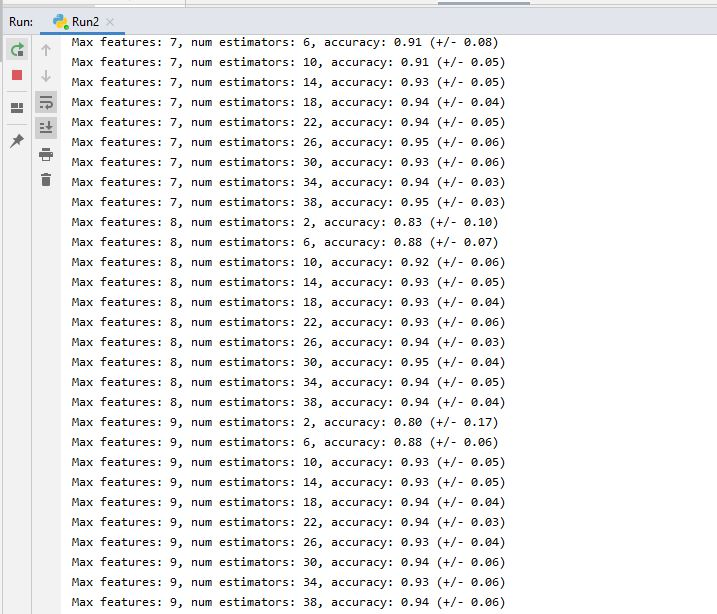
\includegraphics[scale=0.5]{figures/1174042/chapter4/2,8.JPG}
\caption{hasil}
\label{Praktek no 8}
\end{figure}

\begin{figure}[ht]
\centering
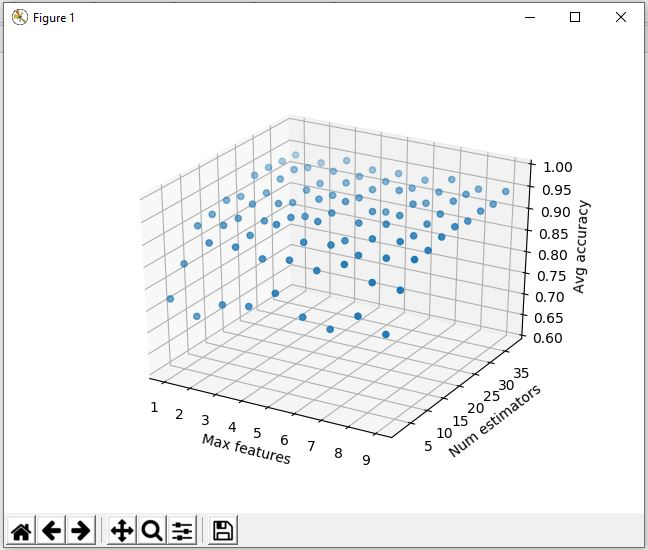
\includegraphics[scale=0.5]{figures/1174042/chapter4/2,8,1.JPG}
\caption{hasil}
\label{Praktek no 8}
\end{figure}
terdapat grafik data yang terdapat dari grafik tersebut di dapat dari codingan dengan cara pengulangan data masing masing 10 kali setelah itu di eksekusi menjadi grafik berbentuk 3D pada gambar tersebut menunjukan rasio dari yang terrendah yaitu data SVM kemudian data decision tree dan hasil random forest.

\end{enumerate}


\subsection{Penanganan Error}
\begin{enumerate}
\item screnn shoot error

\begin{figure}[ht]
\centering
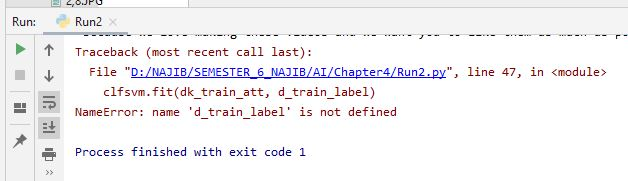
\includegraphics[scale=0.5]{figures/1174042/chapter4/3,1.JPG}
\caption{hasil}
\label{Error}
\end{figure}

\item codingan yang errornya terdapat pada 
\begin{verbatim}
clfsvm.fit(dk_train_att, d_train_label)
\end{verbatim}
\item solusinya
\begin{verbatim}
clfsvm.fit(dk_train_att, dk_train_label)
\end{verbatim}
\end{enumerate}